\documentclass[11pt,a4paper]{article}
% packages
\special{papersize=210mm,297mm}
% package includes
\usepackage{graphicx}
%\usepackage{pslatex}
\usepackage{url}
\usepackage[pdfborder={0 0 0}]{hyperref}
%\usepackage[utf8x]{inputenc}
\usepackage{listings}
\usepackage{color}
\usepackage{cite}
\usepackage{moreverb}
\usepackage{float}
\usepackage{amsmath}
\usepackage{amssymb}
\usepackage{cancel}
% polynomial division
%\usepackage{polynom}
%\usepackage{eucal}
\usepackage{ifthen}
% balkendiagramme
\usepackage{tikz}
\usepackage{tabularx}

% more like the usual word processing dimensions
%\usepackage[top=3cm, bottom=3cm, left=2.54cm, right=2.54cm]{geometry}
\usepackage{bibgerm,cite}
\usepackage{lastpage}
\usepackage{layout}
\usepackage{fancyhdr}
\usepackage{ucs} 
\usepackage[utf8x]{inputenc}
%\usepackage[ngerman,english]{babel}
%\usepackage{scrpage2}
\usepackage{listings} \lstset{numbers=left, numberstyle=\tiny, numbersep=5pt, captionpos=b} 
\usepackage{caption}
\usepackage{algorithm}
\usepackage{algorithmic}
\usepackage{pdflscape}
\usepackage{paralist}
%package includes end
% Settings
\setcounter{secnumdepth}{3}
\setcounter{tocdepth}{3}
\definecolor{listinggray}{gray}{0.9}
\pagestyle{fancy}

\numberwithin{equation}{section} 
%\figurewithin{figure}{section}

% variable to check if specification should be included
\newboolean{INCLUDE_SPEC}
\setboolean{INCLUDE_SPEC}{false}

% macros
\fancyhf{}
\fancyhead[L]{\lvNr\ \lvName}
\fancyhead[R]{\exerciseNr}
\fancyfoot[L]{\authorName, \matrNr, \studNr}
\fancyfoot[C]{- \thepage /\pageref{LastPage} -}
\fancyfoot[R]{\semester}

\newcommand{\HRule}{\rule{\linewidth}{0.5mm}}
\newenvironment{frcseries}{\fontfamily{stix}\selectfont}{}

\newcommand{\textfrc}[1]{{\frcseries#1}}
\newcommand{\mathfrc}[1]{\text{\textfrc{#1}}}

\renewcommand{\algorithmicrequire}{\textbf{Input:}}
\renewcommand{\algorithmicensure}{\textbf{Result:}}

% titlepage macros
\newcommand{\lvNr}{185.A51}
\newcommand{\lvName}{PPMRob}
\newcommand{\semester}{SS12}
\newcommand{\exerciseNr}{2}
\newcommand{\exerciseName}{line detection}

\newcommand{\authorName}{Eugen Dahm}
\newcommand{\matrNr}{0625325}
\newcommand{\studNr}{534}
\newcommand{\mailAddr}{e0625325@student.tuwien.ac.at}

% OPTIONAL
%\newcommand{\groupNr}{swa043}

% OPTIONAL URL
%\newcommand{\optional}{\href{www.flickr.com}{www.flickr.com}}
% authorList for group assignments
\newcommand{\authorList}{
%  \authorNameP, \matrNrP, \studNrP\\ [0.15cm]
%  \authorNameF, \matrNrF, \studNrF\\ [0.15cm]
%  \authorNameM, \matrNrM, \studNrM\\ [0.15cm]
%  \authorNameH, \matrNrH, \studNrH\\ [0.15cm]
  \authorName, \matrNr, \studNr
}

%%% Local Variables:
%%% mode: latex
%%% TeX-master: "../template"
%%% End:

\begin{document}  
% title Page
%\renewcommand \thesection {\arabic{section}.}
\begin{titlepage}
 
\begin{center}
 
% Upper part of the page
%  \includegraphics[width=0.15\textwidth]{logo1}
%  \includegraphics[width=0.15\textwidth]{logo2}
%  \includegraphics[width=0.15\textwidth]{logo3} \\[2cm]

  \begin{minipage}{0.20\textwidth}
    \begin{flushleft} 
      \lvNr
    \end{flushleft}
  \end{minipage}
  \begin{minipage}{0.50\textwidth}
    \begin{center}
      \textsc{\lvName}
    \end{center}
  \end{minipage}
  \begin{minipage}{0.20\textwidth}
    \begin{flushright}
      \semester
    \end{flushright}
  \end{minipage}
  \\[0.3cm]
  \textsc{\exerciseNr} 
  \\[0.7cm]
% Title
\HRule \\[0.4cm]
{ \huge \bfseries \exerciseName}\\[0.4cm]
 
\HRule \\[2cm]
 
% Author and supervisor

%\begin{minipage}{0.4\textwidth}
%\begin{flushleft} \large
%\emph{Author:}\\
%John \textsc{Smith}
%\end{flushleft}
%\end{minipage}
%\begin{minipage}{0.4\textwidth}
%\begin{flushright} \large
%\emph{Supervisor:} \\
%Dr. Mark \textsc{Brown}
%\end{flushright}
%\end{minipage}

%\vfill

%\Large \textbf{\optional}
\normalsize
\vfill
 
% Bottom of the page
%\large \groupNr \\[12pt]
\large \authorList \\[0.5cm]

{\href{mailto:\mailAddr}{\mailAddr}\\} 
\large \today
\end{center}
\end{titlepage}

%%% Local Variables: 
%%% mode: latex
%%% TeX-master: "../template"
%%% End: 


\newpage
% \setcounter{tocdepth}{1}
\tableofcontents
\thispagestyle{empty}
\clearpage
\pagenumbering{arabic}
\section{Houghlines}

\subsection{hough lines storage File Format}
To store detected lines, we use json :).
Hough lines are stored line based in the following format: 
\\
\{\\
``start\_point'': 
\{``x'':
\textless start x\textgreater, ``y'':\textless start y\textgreater\}, \\
``end\_point'': 
\{``x'':
\textless end x\textgreater, ``y'':\textless end y\textgreater\}
\\
\}

\subsection{road images detected lines}

\begin{figure}[H]
  \centering
  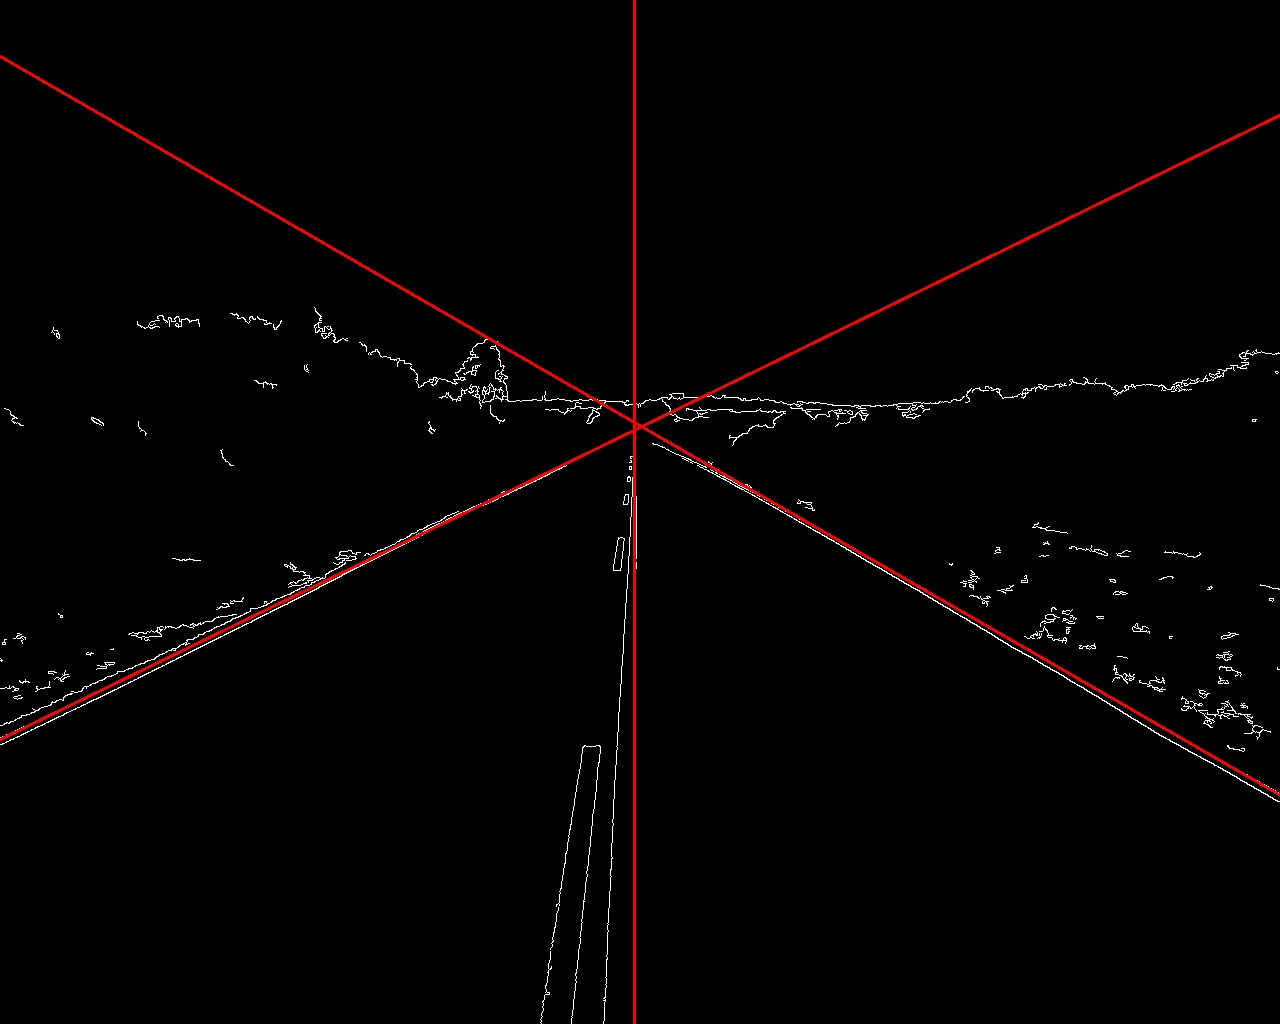
\includegraphics[width=0.6\textwidth]{road_A_canny}
  \caption{road A canny}
  \label{fig:canny_A}
\end{figure}

\begin{figure}[H]
  \centering
  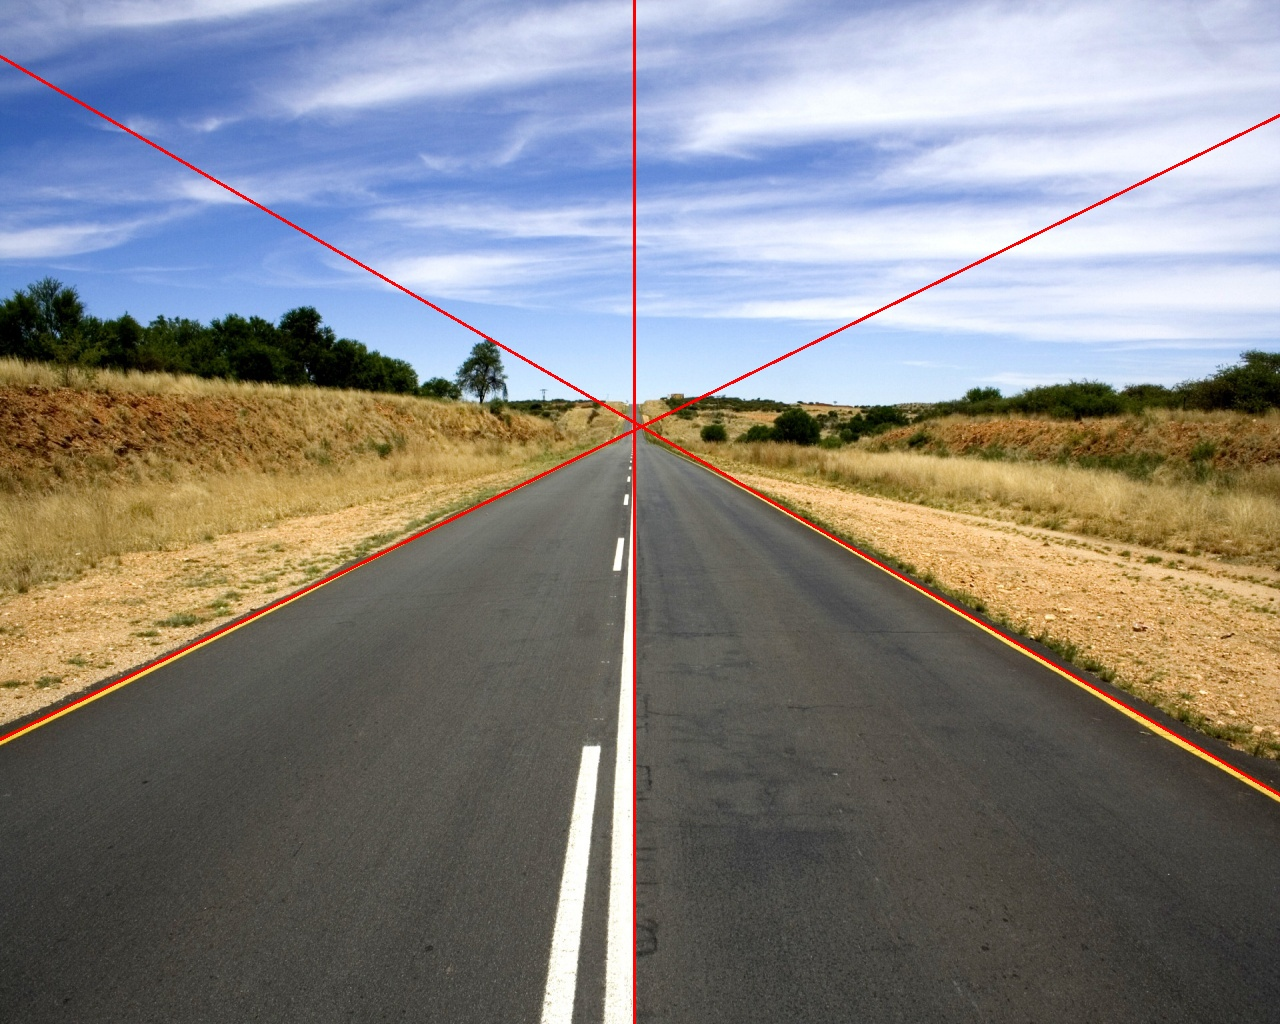
\includegraphics[width=0.6\textwidth]{road_A_horizon}
  \caption{road A final}
  \label{fig:roadA}
\end{figure}

\subsubsection{road B horizon detection}

\begin{figure}[H]
  \centering
  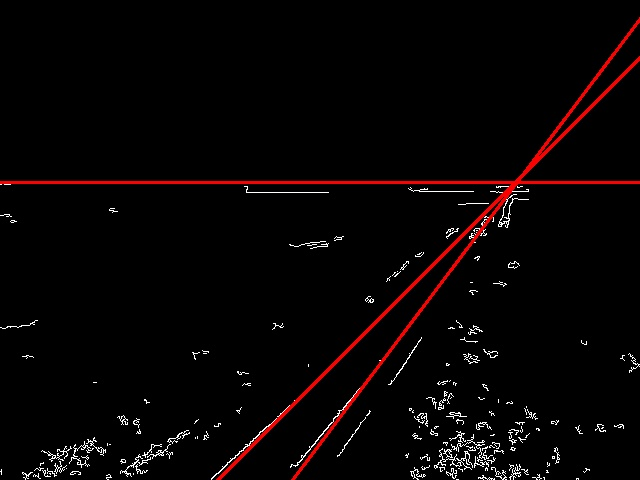
\includegraphics[width=0.9\textwidth]{road_B_canny}
  \caption{road B canny}
  \label{fig:canny_B}
\end{figure}

\begin{figure}[H]
  \centering
  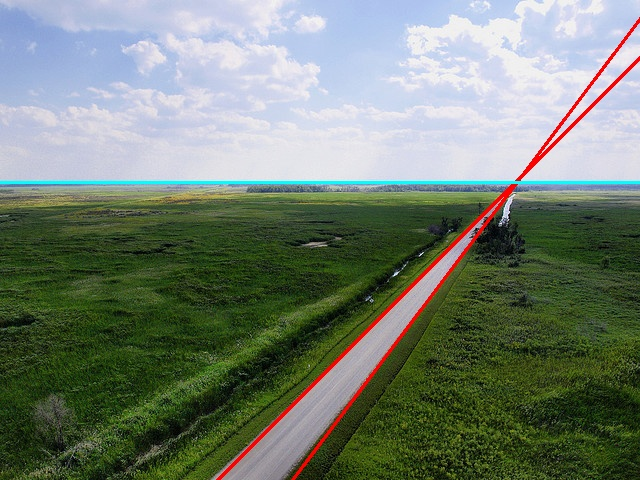
\includegraphics[width=0.9\textwidth]{road_B_horizon}
  \caption{road B with horizon}
  \label{fig:B_horizon}
\end{figure}

\section{houghcircles}

\begin{figure}[H]
  \centering
  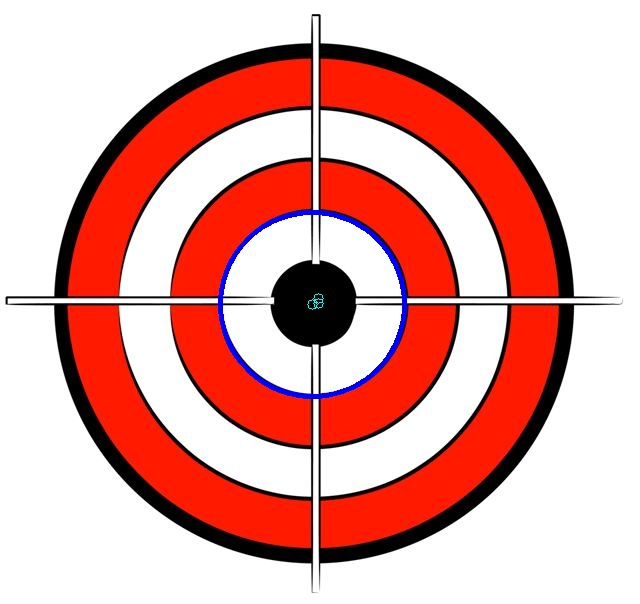
\includegraphics[width=0.72\textwidth]{bullseye_bullseye}
  \caption{bullseye detection via line intersection and circle detection}
  \label{fig:bullseye}
\end{figure}

\begin{figure}[H]
  \centering
  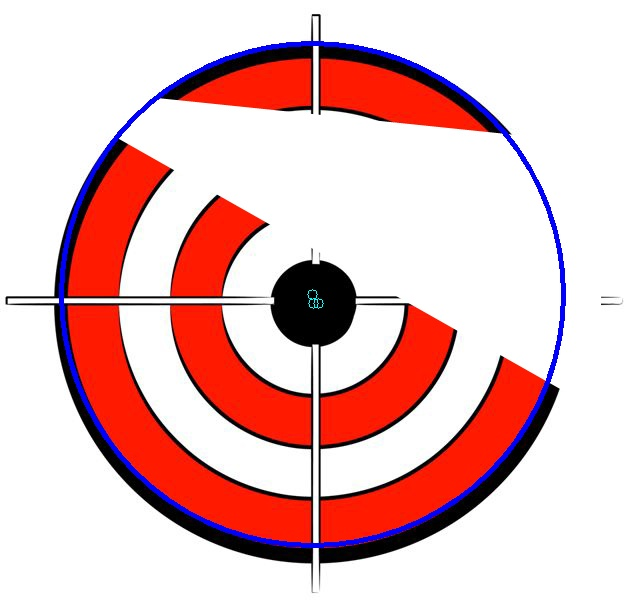
\includegraphics[width=0.72\textwidth]{bullseye_partial_bullseye}
  \caption{partial bullseye detection}
  \label{fig:partial_bullseye}
\end{figure}
\end{document}
